\documentclass[border=10pt]{standalone}
\usepackage{tkz-euclide}

\usepackage{tikz}
\usetikzlibrary{calc,
                intersections,
                arrows.meta
                }

\begin{document}

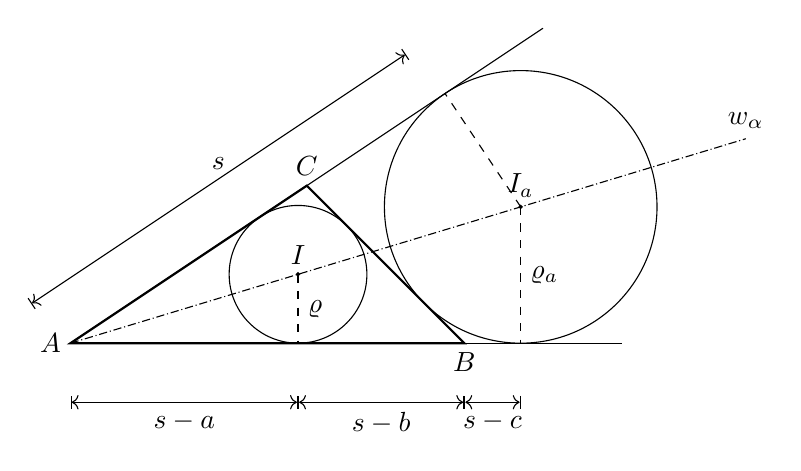
\begin{tikzpicture}
    % Koordinaten der Eckpunkte des Dreiecks
    \coordinate [label=left:$A$] (A) at (0,0);
    \coordinate [label=below:$B$] (B) at (5,0);
    \coordinate [label=above:$C$] (C) at (3,2);

    % Zeichne das Dreieck
    \draw[thick] (A) -- (B) -- (C) -- cycle;

    % Berechne Seitenlängen
    \pgfmathsetmacro{\a}{8^(1/2)}
    \pgfmathsetmacro{\b}{13^(1/2)}
    \pgfmathsetmacro{\c}{5}

    % halber Umfang
    \pgfmathsetmacro{\s}{(\a + \b + \c) / 2}
    % Fläche des Dreiecks
    \pgfmathsetmacro{\A}{5}
    % Inkreisradius
    \pgfmathsetmacro{\rho}{\A / \s}
    % Ankreisradius
    \pgfmathsetmacro{\rhoa}{\A / (\s - \a)}
    
    % Zeichne den Inkreis
    \coordinate [label=above:$I$] (I) at (\s-\a,\rho);
    \draw (I) circle (0.2mm);
    \draw (I) circle (\rho);

    % Zeichne den Ankreis a
    \coordinate [label=above:$I_a$] (Ia) at (3*\s-\c-\b-\a, \rhoa);
    \draw (Ia) circle (0.2mm);
    \draw (Ia) circle (\rhoa);

    % Zeichne Winkelhalbierende alpha
    \draw[add= 0 and 0.5, densely dash dot] (A) to node[at end, above]
    {$w_{\alpha}$} (Ia);
    % Zeichne Basislinie
    \draw (A) to (7,0);
    % Zeichne Linie entlang der Seite b
    \draw[add= 0 and 1] (A) to (C);

    % Zeichne die Hilfslinie für s-Bruchteile
    \draw[|<->|] (0,-.75) -- node[below] {$s-a$} (\s-\a,-.75);
    \draw[|<->|] (\s-\a,-.75) -- node[below] {$s-b$}
    (5,-.75);
    \draw[|<->|] (5,-.75) -- node[below] {$s-c$} (3*\s-\c-\b-\a,-.75);

    % Zeichnen der Linien zu den Fusspunkten
    \coordinate (Fi)  at (\s-\a, 0);
    \coordinate (Fia) at (3*\s-\c-\b-\a, 0);
    \draw[dashed, thin] (I) -- node[right] {$\varrho$} (Fi);
    \draw[dashed, thin] (Ia) -- node[right] {$\varrho_a$} (Fia);

    \coordinate (Fiao) at ($(A)!(Ia)!(C)$);
    \draw[dashed, thin] (Ia) -- (Fiao);

    % Zeichne Hilfsline s
    \draw[|<->|] ($(A)+(-5mm,5mm)$) -- node[above] {$s$} ($(Fiao)+(-5mm,5mm)$);
   
\end{tikzpicture}

\end{document}